%! Author = antonio
%! Date = 7/2/24

Logistic Regression is a discriminative classification model, directly evaluating the posterior probability \(C \mid X\).
In particular by determining that hyperplane which maximises the posterior probability.
Starting from the results obtained from the Tied Gaussian that provides log-likelihood ratios that are linear functions
of our data, where log-posterior probability ratio is:

\begin{equation}
    \log \frac{P(C=h_1 \mid X)}{P(C=h_0 \mid X)} = \log \frac{f_{X \mid C}(x \mid h_1)}{f_{X \mid C}(x \mid h_0)} + \log \frac{\pi}{1-\pi} = \omega^T x + b
    \label{eq:logisticRegression}
\end{equation}

where prior information has been absorbed in the bias term \(b\) of the \autoref{eq:logisticRegression}.
So from this point we can define the score function as:

\begin{equation}
    s(x) = \omega^T x + b = 0
    \label{eq:scoreFunctionLR}
\end{equation}

where it is positive for samples of class \(h_1\) and negative for samples of class \(h_0\).
Given \(\omega\) and \(b\) we can compute the posterior class probability as:

\begin{equation}
    P(C=h_1 \mid x, \omega, b) = \sigma(\omega^T x + b) = \sigma(s(x))
    \label{eq:posteriorClassProbabilityLR}
\end{equation}
where \(\sigma\) is sigmoid function defined as:

\begin{equation}
    \sigma(x) = \frac{1}{1 + e^{-x}}
\end{equation}

This approach assumes that the decision rules will be hyperplanes orthogonal to vector w.

\subsubsection{Binary Logistic Regression}
\textbf{Binary Logistic Regression Not Prior-Weighted}\n
The objective is to minimise the loss function \(J(\omega,b)\), but to this is introduced what is a penalty term,
so the new function becomes:

\begin{equation}
    R(\omega,b) = \frac{\lambda}{2}\left\|w \right\|^2 + \frac{1}{n} \sum_{i=1}^{n} \log (1+e^{-z_i(\omega^T x_i + b)}), \quad
    z_i = \begin{cases}
              1 & \text{if } c_i = 1 \\
              -1 & \text{if } c_i = 0
    \end{cases}
    \label{eq:minimiseFunctionLR}
\end{equation}

where \lampda of \autoref{eq:minimiseFunctionLR} is the regularization term, this term has been introduced to make problem
solvable in case of linearly separable classes.

\begin{figure}[h!]
    \centering
    \begin{subfigure}[b]{0.3\linewidth}
        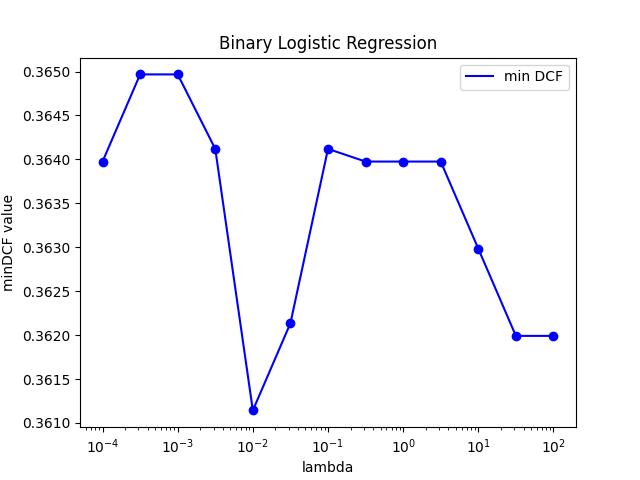
\includegraphics[width=\linewidth]{Lab/08. Lab 08/Images/01. BLR - minDCF}
        \caption{minDCF}
        \label{fig:BLRminDCF}
    \end{subfigure}
    \begin{subfigure}[b]{0.3\linewidth}
        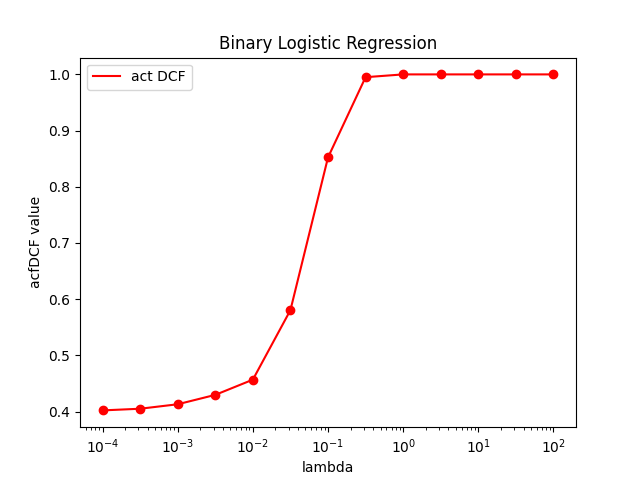
\includegraphics[width=\linewidth]{Lab/08. Lab 08/Images/02. BLR - actDCF}
        \caption{actDCF}
        \label{fig:BLRactDCF}
    \end{subfigure}
    \begin{subfigure}[b]{0.3\linewidth}
        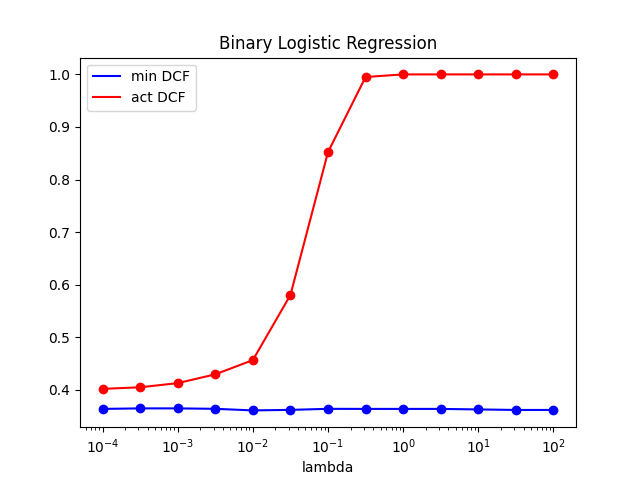
\includegraphics[width=\linewidth]{Lab/08. Lab 08/Images/03. BLR - min And actDCF}
        \caption{minDCF vs actDCF}
        \label{fig:minAndactDCF}
    \end{subfigure}
    \caption{Binary Logistic Regression}
    \label{fig:BLR}
\end{figure}